% ─────────────────────────────────────────────────────────────────────────────
%  SECTION: Technologies Used, Source Code, and AI Tools
% ─────────────────────────────────────────────────────────────────────────────

\section{Technologies Used, Source Code, and Development Tools}

% ─── 4.1 Technologies Used ──────────────────────────────────────────────────
\subsection{Technologies Used}

The technology choices for \textbf{AgriGov Market} were not arbitrary; each tool was selected for a concrete technical reason aligned with the project's requirements. The full stack is summarised below, followed by a justification for each choice.

\begin{itemize}
	
	\item \textbf{Programming Languages:}
	\begin{itemize}
		\item \textbf{Python} (backend) — chosen for its readability, its mature ecosystem of web and data libraries, and its first-class support in the Django framework \cite{VanRossumDrake2009}.
		\item \textbf{TypeScript} (frontend) — a statically typed superset of JavaScript that catches type errors at compile time, which improves reliability and maintainability when working with complex API response objects \cite{MicrosoftTypeScript2024}.
	\end{itemize}
	
	\item \textbf{Frameworks:}
	\begin{itemize}
		\item \textbf{Django} (backend) — a high-level Python web framework that enforces the MVT architectural pattern and provides built-in modules for authentication, ORM-based database access, and security. Its companion library \textbf{Django REST Framework (DRF)} was used to expose the application's functionality as a RESTful API, handling serialization, routing, and permission policies \cite{DjangoProject2024,Christie2024DRF}.
		\item \textbf{Next.js} (frontend) — a React-based framework developed and maintained by Vercel. It was preferred over a plain React application because it provides server-side rendering (SSR) and static generation out of the box, which improves initial page-load performance and SEO. Its App Router also supports clean, file-based routing that maps naturally onto the platform's multi-role structure \cite{Vercel2024Nextjs}.
	\end{itemize}
	
	\item \textbf{Database:} \textbf{PostgreSQL} — a production-grade, open-source relational database system. It was selected over lighter alternatives (such as SQLite) because the platform's data model involves multiple related entities (users, products, orders, deliveries, transport assignments) with strict referential integrity constraints. PostgreSQL's support for transactions, foreign keys, and indexing made it the appropriate choice \cite{PostgreSQLGroup2024}.
	
	\item \textbf{Database Hosting:} \textbf{Neon} — a serverless PostgreSQL hosting service that provides a cloud-managed database with automatic scaling and branching support. It removes the overhead of managing a database server manually, which is valuable in an academic development context where infrastructure simplicity is a priority \cite{NeonTech2024}.
	
	\item \textbf{File Storage:} \textbf{Cloudinary} — a cloud-based media management platform used to upload, store, and serve product images and other media files. Rather than storing binary files directly in the database or on the application server (which would complicate deployment and degrade performance), Cloudinary offloads media delivery to a CDN, ensuring fast image loading regardless of the user's location \cite{Cloudinary2024}.
	
	\item \textbf{Styling:} \textbf{Tailwind CSS} — a utility-first CSS framework that enables rapid construction of responsive interfaces without writing custom stylesheets. It was chosen to accelerate frontend development and maintain visual consistency across components \cite{TailwindLabs2024}.
	
	\item \textbf{Development Environment:} \textbf{Visual Studio Code} — a lightweight but feature-rich code editor with strong support for Python, TypeScript, Git integration, and extensions for Django and React development \cite{Microsoft2024VSCode}.
	
	\item \textbf{Version Control:} \textbf{Git and GitHub} — used to manage the codebase, track changes, and coordinate work between team members through branches and pull requests \cite{Chacon2014ProGit}.
	
\end{itemize}

% ─── 4.2 AI Tools Used in Development ──────────────────────────────────────
\subsection{AI Tools Used in Development}

Artificial intelligence assistants were integrated into the development workflow as productivity and quality tools. Their use was transparent and complementary to the team's own design and engineering decisions; all generated outputs were reviewed, adapted, and validated before integration into the project.

\subsubsection{ChatGPT (OpenAI)}

\textbf{ChatGPT} \cite{OpenAI2024ChatGPT}, developed by OpenAI, is a large language model (LLM) conversational assistant. In this project it was used for:

\begin{itemize}
	\item \textbf{Code generation and debugging:} generating boilerplate code for Django models, DRF serializers and views, as well as diagnosing errors in Python and TypeScript.
	\item \textbf{Query optimisation:} suggesting improvements to PostgreSQL queries and Django ORM calls to reduce redundant database hits.
	\item \textbf{Documentation:} assisting in the drafting of inline code comments and API endpoint descriptions.
\end{itemize}

\subsubsection{Claude (Anthropic)}

\textbf{Claude} \cite{Anthropic2024Claude}, developed by Anthropic, is a large language model assistant oriented toward long-context reasoning and document understanding. In this project it was used for:

\begin{itemize}
	\item \textbf{Architecture review:} discussing design choices — such as the separation between the Django backend and the Next.js frontend — and validating that the chosen patterns were appropriate for the project's scale.
	\item \textbf{Technical writing:} improving the clarity, structure, and academic tone of this thesis, including the introductions, conclusions, and this section.
	\item \textbf{Refactoring suggestions:} reviewing sections of backend code and proposing more maintainable alternatives aligned with Django best practices.
\end{itemize}

\subsubsection{Ethical and Academic Considerations}

The use of AI tools in this project complies with the transparency principle recommended by several academic institutions \cite{Perkins2023AIAcademic}: all AI-assisted content was critically evaluated and rewritten where necessary, no AI tool was used as a substitute for the team's own understanding of the system, and all design decisions remained the intellectual responsibility of the authors. The AI tools were used as an assistant, not as an author.

% ─── 4.3 Source Code Description ────────────────────────────────────────────
\subsection{Source Code Description}

This section describes the organisation of the application's source code.

\paragraph{Project Structure}
The backend is organised into multiple Django applications, each representing a distinct domain of the system (users, products, orders, transport). This modular structure limits coupling between functional areas and makes it straightforward to extend or modify a single domain without affecting others.

\begin{figure}[H]
	\centering
	\begin{subfigure}[b]{0.3\textwidth}
		\centering
		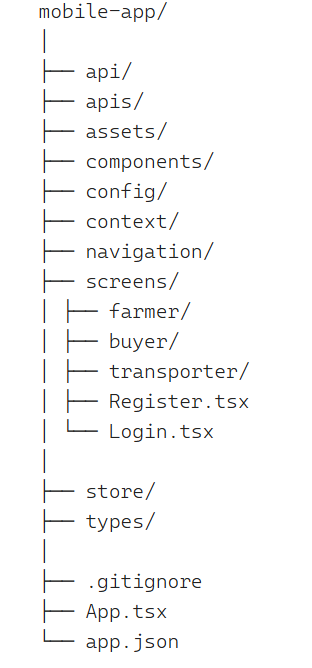
\includegraphics[width=\textwidth]{images/structure/mobileStructure}
		\caption{Mobile Structure}
	\end{subfigure}
	\hfill
	\begin{subfigure}[b]{0.3\textwidth}
		\centering
		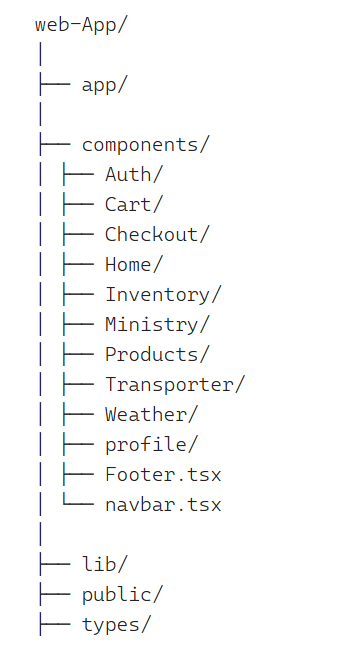
\includegraphics[width=\textwidth]{images/structure/webStructure}
		\caption{Web Structure}
	\end{subfigure}
	\hfill
	\begin{subfigure}[b]{0.3\textwidth}
		\centering
		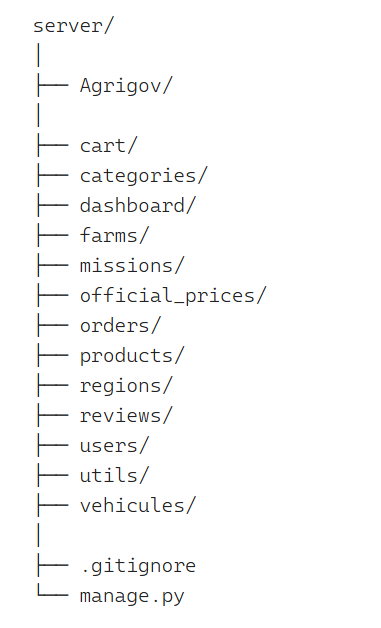
\includegraphics[width=\textwidth]{images/structure/backendStructure}
		\caption{Backend Structure}
	\end{subfigure}
	\caption{Overall Project Structure}
\end{figure}

At the root level, the project includes configuration files such as \texttt{manage.py}, environment variables (\texttt{.env}), and dependency definitions (\texttt{requirements.txt}).

\paragraph{Main Components}
Each Django application within the backend is composed of four primary building blocks:

\begin{itemize}
	\item \textbf{Models:} Define the database schema and entity relationships using Django's ORM, eliminating the need to write raw SQL for standard operations.
	\item \textbf{Views:} Handle incoming HTTP requests, apply business logic, interact with models, and return structured API responses via DRF.
	\item \textbf{Serializers:} Convert model instances into JSON (and vice versa), enforcing field-level validation before data is written to the database.
	\item \textbf{URLs:} Map API endpoints to their corresponding view functions or viewsets, defining the public interface of each application.
\end{itemize}

\paragraph{Logical Organisation: MVT Architecture}
The backend follows the \textbf{Model–View–Template (MVT)} pattern native to Django \cite{DjangoProject2024}. In this project, the Template layer is replaced by the Next.js frontend, which consumes the REST API and handles all rendering. This decoupling has three concrete benefits:

\begin{itemize}
	\item The backend and frontend can evolve independently — a mobile client (React Native) can consume the same API without any changes to the backend.
	\item The frontend benefits from Next.js's server-side rendering capabilities, which would not be possible if HTML were generated by Django templates.
	\item Testing is simplified: backend logic can be unit-tested without a browser, and frontend components can be tested in isolation.
\end{itemize}

% ─── 4.4 Repository Access ──────────────────────────────────────────────────
\subsection{Access to the Project Repository}

The complete source code is publicly available at the following repositories:

\begin{itemize}
	\item \textbf{Web Frontend \& Backend:} \url{https://github.com/DabbacheDjawad/AGRIGOV-MARKET.git}
	\item \textbf{Mobile Application:} \url{https://github.com/BenhamadaKhalil/Agrigov-mobile.git}
\end{itemize}

\begin{figure}[H]
	\centering
	{\color{black}\qrcode[height=7cm]{https://github.com/BenhamadaKhalil/agrigov-bachelor-thesis/tree/main/images/QR}}
	\vspace{0.6cm}
	
	\textbf{Scan to access additional downloadable content}
\end{figure}

